\section{Fourier and Laplace}

Some qualitative intuition before we begin.
The Fourier transform scans a signal for sinusoidal terms.
The Laplace transform does the same, but \emph{also} scans the signal for exponential terms.
That's why the latter is so popular in differential equations: many differential equations have solutions that contain both sinusoidal and exponential terms. 


\begin{figure}[H]
  \caption{Time Base versus Fourier Base}
  \centering
    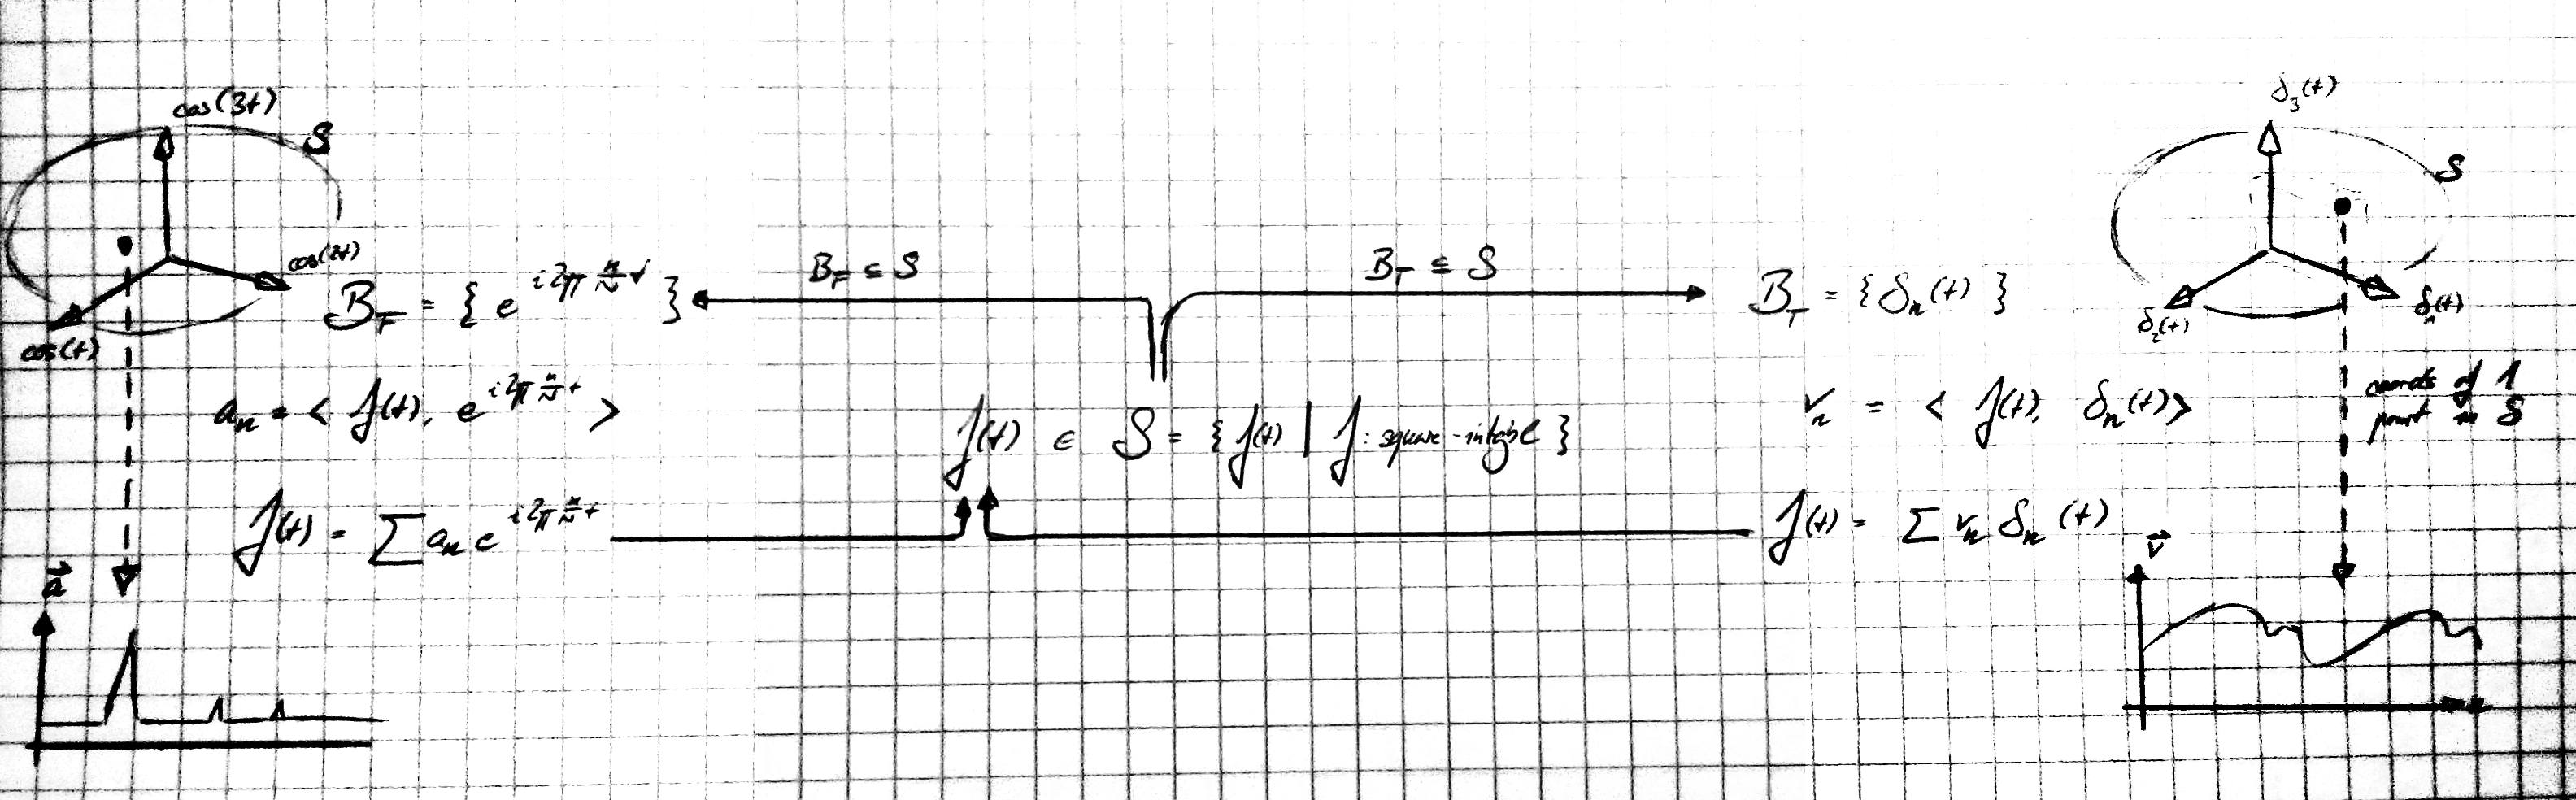
\includegraphics[width=0.95\textwidth]{images/fourier_base.jpg}
\end{figure}


\subsection{Discrete Fourier Analysis}

We'll begin with the discrete case. For one, this case is the basis of the FFT. Also, the math is a lot easier in the discrete case.
Let $N$ be the sample-size and $\delta$ be the sample-frequency (often equal to 44100 Hz or 48000 Hz).
Let $V$ be the sample-space of signals of size $N$. This is a vector-space,
equipped with an inner product of the form $\innerprodbr{\vec{a}}{\vec{b}} = \frac{1}{N} \sum_{k=0}^{N-1} a_k (b_k)^*$,
where $()^*$ is the complex complement.

\subsubsection{The Fourier Base}




We'll use the base $B = \{ \vec{w}_N^n | n \in [0, N-1]\}$. Here, $\vec{w}_N^n$ is the vector we get
by evaluating $e^{i 2\pi \frac{n}{N} k}$ at the points $k=0, k=1, ..., k=N-1$.
Thus if we call $w_N = e^{i 2 \pi \frac{1}{N}}$, then the vector $\vec{w}_N^n$ consists of the elements $w_N^{nk}$.
Throughout this chapter, $k$ will be the index of time/the signal-vector and $n$ will be the index of frequency/the base-vectors.

In the case of $N = 4$ we obtain the matrix:
$$ \left[\begin{matrix}e^{0.25 i \pi} & e^{0.5 i \pi} & e^{0.75 i \pi} & e^{1.0 i \pi}\\e^{0.5 i \pi} & e^{1.0 i \pi} & e^{1.5 i \pi} & e^{2.0 i \pi}\\e^{0.75 i \pi} & e^{1.5 i \pi} & e^{2.25 i \pi} & e^{3.0 i \pi}\\e^{1.0 i \pi} & e^{2.0 i \pi} & e^{3.0 i \pi} & e^{4.0 i \pi}\end{matrix}\right] $$
Note that Fourier-bases are symmetric matrices. 

The Fourier-base is a very particular choice: each element of each base-vector turns out to be one of the $N$ complex $N$th roots of one. We could have chosen any base-vectors, but these complex roots will turn out to have a few useful properties that we will exploit to speed up the Fourier transformation. These properties are:

\begin{enumerate}
    \item $w_N^x = (w_N)^x$
    \item $w_N^{2x} = w_{N/2}^x$
    \item $w_N^{2x+N} = w_N^{2x}$
    \item $w_N^{x+N/2} = - w_N^x$
\end{enumerate}

It is also easy to prove that this base is orthogonal.
\begin{proof} The vectors $\vec{w}_N^n$ are orthogonal. \\
\subprf{Suppose $n \neq m$.}
    {$\innerprodbr{\vec{w}_N^n}{\vec{w}_N^m} = 0$ }{
    
    $\innerprodbr{\vec{w}_N^n}{\vec{w}_N^m} = \frac{1}{N} \sum_{k=0}^{N-1} e^{i 2\pi \frac{n-m}{N} k} $ \\
    
    Using the result $\sum_{n=0}^{N-1} e^{xn} = \frac{1-e^{xN}}{1-e^{x}}$, we find: \\
    
    $\frac{1}{N} \sum_{k=0}^{N-1} e^{i 2\pi \frac{n-m}{N} k} = \frac{1}{N} \frac{1-e^{i 2\pi (n-m)}}{1-e^{i 2\pi \frac{n-m}{N}}}$ \\
    
    It is easy to see that $e^{i 2\pi (n-m)} = 1$. So the above term must equal 0.
    
    
}
\subprf{Suppose $n = m$.}
    {$\innerprodbr{\vec{w}_N^n}{\vec{w}_N^m} = 1$ }{

    We use the same line of reasoning as above to obtain: \\
    
    $ \innerprodbr{\vec{w}_N^n}{\vec{w}_N^m} = \frac{1}{N} \frac{1-e^{i 2\pi (0)}}{1-e^{i 2\pi \frac{0}{N}}}$ \\
    
    In the limit, this equals 1.
}
\end{proof}


Proof of spanning

\subsubsection{Obtaining the amplitudes}
After having proven that $B$ is an orthonormal base for $V$, we can get to the core of the Fourier analysis:
given a signal $\vec{v}$, how do we obtain the amplitudes in $\vec{v} = \sum_{n=0}^{N-1} \alpha_n \vec{w}_n$ ?
Well, from paragraph \ref{fourierDecomposition} we know that 

$$ \alpha_n = \innerprodbr{\vec{v}}{\vec{w}_N^n} = \frac{1}{N} \sum_{k=0}^{N-1} v_k e^{i 2\pi \frac{n}{N} k} $$

Using Horner's method, this is a \BigTheta{n} operation.
Executing it on all $n$ coefficients, the whole process becomes a \BigTheta{n^2} operation.
A naive implementation might look like this: 

\begin{lstlisting}[language=python]
import numpy as np

def amplitudes(signal):
    N = len(signal)
    amps = []
    for n in range(N):
        sm = 0
        for k in range(N):
            wnk = np.exp(-1j * 2 * np.pi * n * k / N) 
            sm += signal[k] * wnk
        amps.insert(n, sm/N)
    return amps


sig = [2, 1, 1, 4]
print amplitudes(sig)
\end{lstlisting}

Notice that this is a matrix operation. 


\subsection{As a matrix operation}

\begin{proof}
    The Fourier transform of $\vec{a} + \vec{b}$ equals the transform of $\vec{a}$ plus the transform of $\vec{b}$

    Note that the Fourier transform can be rewritten in matrix form. 
    
    $$
    <\vec{a}, \vec{f}_m>(m) = 
    \begin{bmatrix} f_{1,1} & ... & f_{F,T} \\ ... & & ... \\ f_{F,1} & ... & f_{1,T}  \end{bmatrix} 
    \begin{bmatrix} a_1 \\ a_2 \\ ... \\ a_T \end{bmatrix}  
    = 
    \begin{bmatrix} <\vec{a}, \vec{f}_1> \\ <\vec{a}, \vec{f}_2> \\ ...  \\ <\vec{a}, \vec{f}_F> \end{bmatrix} 
    $$
    
    This means that the rules for matrix multiplication apply to the Fourier transformation, amongst which that matrix multiplication is distributive:
    
    $$ A (\vec{a} + \vec{b}) = A \vec{a} + A \vec{b} $$
    
    Remember that a matrix-multiplication is always a change of basis:
    the vector $\vec{v}_I$ (as displayed in the Euclidean system $\mtrx{I}$) can also be expressed
    relative to the Fourier-base $\mtrx{F}$ as $\vec{v}_F$. 
    $$ \mtrx{F}^{-1} \vec{v}_I = \vec{v}_F $$
    where (according to \ref{changeOfBasis}): 
    $$ \mtrx{F}^{-1} = \begin{bmatrix} \vec{x}_F & \vec{y}_F & \vec{z}_F \end{bmatrix} $$
    
\end{proof}


\subsection{Fast Fourier Transform}

In the previous section we have evaluated the polynomial $\sum_{k=0}^{N-1} v_k e^{i 2 \pi \frac{n}{N} k}$ like this:
\begin{lstlisting}[language=python]
for k in range(N):
    wnk = np.exp(1j * 2 * np.pi * n * k / N) 
    sm += signal[k] * wnk
\end{lstlisting}

Really, this is just the same as evaluating the polynomial $A(x) = \sum_{k=0}^{N-1} v_k x^k$, where $x = e^{i 2 \pi \frac{n}{N} 1} = w_N^n$ (using property 1). In other words, we calculated $A(w_N^n)$.

However, it turns out that we can simplify this process. Before we detail how exactly this section is to be simplified, we need to realize that for any polynomial $A(x)$, it holds that $A(x) = A_{even}(x^2) + x A_{odd}(x^2)$


Knowing that, we can split the evaluation in half:
$$ A(w_N^n) = A_{even}(w_N^{2n}) + w_N^n A_{odd}(w_N^{2n})$$


And using the properties 2-4 of $w_N^n$, we can calculate:
\begin{equation} 
\begin{split} 
    A(w_N^n) & = A_{even}(w_N^{2n})   + w_N^n A_{odd}(w_N^{2n})   \\
             & = A_{even}(w_{N/2}^n)  + w_N^n A_{odd}(w_{N/2}^n)
\end{split}
\end{equation}

\begin{equation} 
\begin{split}  
A(w_N^{n + N/2})  & = A_{even}(w_N^{2n+ N}) + w_N^{n+N/2} A_{odd}(w_N^{2n + N}) \\
                  & = A_{even}(w_N^{2n}) - w_N^n A_{odd}(w_N^{2n})   \\
                  & = A_{even}(w_{N/2}^n) - w_N^n A_{odd}(w_{N/2}^n)
\end{split}
\end{equation}

This way, we obtain:
\begin{lstlisting}[language=python]
def fft(signal):
    N = len(signal)

    if N == 1:
        return signal

    sigE = []
    sigU = []
    for k in range(N):
        if k%2 == 0:
            sigE.append(signal[k])
        else:
            sigU.append(signal[k])

    ampsE = fft(sigE)
    ampsU = fft(sigU)

    amps = []
    for n in range(N/2):
        wn = np.exp(-1j * 2 * np.pi * n / N)
        an   = ampsE[n] + wn * ampsU[n]
        an2N = ampsE[n] - wn * ampsU[n]
        amps.insert(n,       an   )
        amps.insert(n + N/2, an2N )

    return amps
\end{lstlisting}

\subsubsection{Backtransformation}

\subsection{Fourier for musical frequencies}
Musical notes are special. Here, we don't want to get the full spectrum that FFT delivers, but only a few selected frequencies. 
\subsubsection{Goertzel}
Goertzel continues to work with the Fourier base. It differs from FFT in that only a few of the elements that FFT returns are actually evaluated. 
\subsubsection{PCI}
PCI (pre-calculated inverse algorithm) discards of the Fourier base and instead uses the musical frequencies in the base.
This results in a non-orthogonal base, but that won't hinder us. 
\begin{equation}
    \begin{split}
        \vec{s} &= \sum_F a_f e^{-2 \pi i f t} \text{  , with F = \{440, 465, ...\}}  \\
                &= \begin{bmatrix}  ... & & ... \\ & e^{- 2 \pi i f t} & \\ ... &  & ... \end{bmatrix} \vec{a} \\
        \vec{a} &= \begin{bmatrix}  ... & & ... \\ & e^{- 2 \pi i f t} & \\ ... &  & ... \end{bmatrix}^{-1} \vec{s}
    \end{split}
\end{equation}

\subsection{Continuous Fourier Analysis}

In Fourier analysis, we deal with the inner-product space $C_{[a,b]}^2$:
the space of square-integrable functions that are continuous from $a$ to $b$.
An orthogonal base for this vector-space would be the Fourier base $\{ sin(\frac{j 2 \pi}{b-a} t), cos(\frac{j 2 \pi}{b-a}  t) | j \in \naturals \}$.
Often, making use of Euler's formula, we instead write this base as $\{ e^{i \frac{n 2 \pi}{b-a} t} | j \in \naturals \}$. 

\subsubsection{Comparing Fourier to other important series}

\paragraph{Fourier versus Taylor} Another famous expansion of functions is the Taylor-expansion.
It is important to note that the Taylor expansion is a completely different beast from the Fourier expansion.

\begin{itemize}
    \item Taylor works on locally differentiable functions, whereas Fourier works on globally integrable functions. 
    You cannot recover the full function from its Taylor-expansion.
    \item The Taylor-base is non-orthogonal\footnote{proof required}
\end{itemize}

\begin{table}[ht]
\centering
\caption{Fourier versus Taylor}
\begin{tabular}{@{}lll@{}}
\toprule
        & coefficients                                              & base-vectors                      \\ \midrule
Fourier & $f(t) \innerprod e^{i \frac{n 2 \pi}{b-a} t}$             & $e^{i \frac{n 2 \pi}{b-a}  t}$    \\
Taylor  & $f^{(n)}(t)|t_0$                                          & $\frac{(x- x_0)^n}{n!}$          
\end{tabular}
\end{table}

\paragraph{Fourier versus PCA} PCA comes a lot closer to Fourier in that in PCA we represent our data as a linear combination of orthogonal base-vectors
 There are two differences though. In PCA the data is usually a matrix instead of a vector. And in PCA we don't know in advance
 what the set of base-vectors is going to be, but much rather chose the most fitting one for our data-matrix.
 It turns out that we can use the set of eigenvectors of the data-matrix\footnote{Strictly speaking, we don't work with the raw data-matrix, but rather its correlation matrix.
 This is because for the eigenvector thing to work , we need the matrix to be symmetric and centered around the origin, which the raw data matrix usually isn't.}.

\begin{proof}There is a set of eigenvectors $E$ of a matrix $M$ that is an orthogonal basis for $\solspace{M}$
    \subprf{}{}{}
\end{proof}

Fourier analysis is often a lot better at compressing. The below image has been created with only 321 frequencies out of a 119*95 image.
\begin{lstlisting}[language=python]
def compressImage(image, threshold):
    freqs = fft.rfft2(image)
    mags = np.abs(freqs)
    thresholdValue = threshold * np.max(mags)
    indices = mags >= thresholdValue
    freqsFiltered = freqs * indices
    imageRestored = fft.irfft2(freqsFiltered)

    print("entries above threshold: " + str(np.count_nonzero(indices)))
    return imageRestored

image = imageio.imread(files[0])
restored = compressImage(image, 0.003)

fix, axes = plt.subplots(1, 2)
axes[0].imshow(image)
axes[1].imshow(restored)
\end{lstlisting}

\begin{figure}[h]
    \caption{Image restored from top 321 frequencies after Fourier transform}
    \centering
      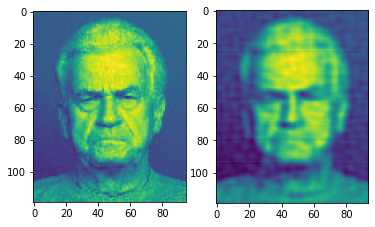
\includegraphics[width=0.5\textwidth]{images/fourier_compression.png}
\end{figure}


\subsubsection{Proving that Fourier functions form a basis}

We can use Fourier to describe any function-space - if we can prove that the Fourier functions do indeed form a basis for that space.
This takes two steps: proving orthogonality and proving span.

\paragraph{Orthogonality} This is very straightforward: 

\paragraph{Span} This  requires more work.  We're first going to have to prove The Weierstrass-Theorem.
This theorem states that the set $B = \{ x^j | j \in \naturals \}$ forms a basis for $C_{[a,b]}$.
https://psychedai.wordpress.com/2016/11/15/the-intuition-behind-bernsteins-proof-of-the-weierstrass-approximation-theorem/


\subsubsection{Fourier transform on vector valued functions}
As long as a vector-valued function can be decomposed over a set of basis-vectors
(never mind what basis vectors exactly, this works with any basis),
we can still use the normal, scalar Fourier transform on them. 
\begin{equation}
    \begin{split}
        g &: A^N \to A^M \\
        g(\vec{x}) &= \sum_m^M g_m(\vec{x}) \vec{e}_m \text{ ... decomposing the function over the output basis} \\
        \fourier_g(\vec{u}) &= \sum_m^M \vec{e}_m \fourier_{g_m}(\vec{u})  \text{ ... Fourier transform over the input basis}
    \end{split}
\end{equation}

Consider the example of a rgb-image.
\begin{equation}
    \begin{split}
        c(x,y) &= \vec{e}_1 r(x,y) + \vec{e}_2 g(x,y) + \vec{e}_3 b(x,y) \\
        \fourier_c\begin{bmatrix} f_x \\ f_y \end{bmatrix} 
                        &= \int_X \int_Y c(x,y) e^{-2\pi i (f_xx + f_yy)} \diff{y} \diff{x} \\
                        &= \int_X \int_Y \vec{e}_1 r(x,y) e^{-2\pi i (f_xx + f_yy)} \diff{y} \diff{x} + ... \\
                        &= \vec{e}_1 \fourier_r\begin{bmatrix} f_x \\ f_y \end{bmatrix} + \vec{e}_2 \fourier_g\begin{bmatrix} f_x \\ f_y \end{bmatrix} + \vec{e}_3 \fourier_b\begin{bmatrix} f_x \\ f_y \end{bmatrix} 
    \end{split}
\end{equation}

Note that the resulting fourier spectrum consist of complex 3d-vectors.

Sometimes, however, you either have an input function that contains \emph{multi-vector} elements,
or you want to apply a filter to the fourier spectrum based on multi-vectors.
In that case, you can find an introduction to geometric-algebra Fourier transforms here: 
\inlinecode{https://pdfs.semanticscholar.org/41ce/67428ee60748a4142dee0eea28ed997855e6.pdf}



\subsection{Fourier Transforms and Convolutions}
One major reason that Fourier transforms are so important in image processing is the convolution theorem which states that

If $f(x)$ and $g(x)$ are two functions with Fourier transforms $F(u)$ and $G(u)$,
then the Fourier transform of the convolution $f(x)*g(x)$ is simply the product of the Fourier transforms of the two functions, $F(u) G(u)$.

Thus in principle we can undo a convolution. e.g. to compensate for a less than ideal image capture system:

\begin{itemize}
	\item Take the Fourier transform of the imperfect image,
	\item Take the Fourier transform of the function describing the effect of the system,
	\item Divide the former by the latter to obtain the Fourier transform of the ideal image.
	\item Inverse Fourier transform to recover the ideal image.
\end{itemize}
This process is sometimes referred to as de-convolution.

\begin{table}[]
    \begin{tabular}{@{}llll@{}}
    \toprule
                                &             & 1D                                                                              & 2D                                                \\ 
    \midrule
    \multirow{2}{*}{continuous} & Transform   & $\fourier_f(u)  = \int_{-\infty}^{\infty} f(t) e^{-2\pi i t u} \diff t$         & $\fourier_f(u, v)  = \int_{-\infty}^{\infty} \int_{-\infty}^{\infty} f(x, y) e^{-2\pi i (ux + vy)} \diff x \diff y$         \\
                                & Convolution & $(f * g)(t)     = \int_{-\infty}^{\infty} f(u) g(t-u) \diff u$                  & $(f * g)(x, y)     = \int_{-\infty}^{\infty} \int_{-\infty}^{\infty} f(u, v) g(x-u, y-v) \diff u \diff v$                      \\
    \multirow{2}{*}{discrete}   & Transform   & $\fourier_f(u)  = \sum_{-\infty}^{\infty} f(t) e^{-2\pi i t u} $                & $\fourier_f(u, v)  = \sum_{-\infty}^{\infty} \sum_{-\infty}^{\infty} f(x, y) e^{-2\pi i (ux + vy)} $                \\
                                & Convolution & $(f * g)(t) = \sum{-\infty}^{\infty} f(u) g(t-u) $                              & $(f * g)(x, y) = \sum_{-\infty}^{\infty} \sum_{-\infty}^{\infty} f(u, v) g(x-u, y-v) $                         \\
    \end{tabular}
\end{table}

Motion blur, for example, can be simulated by convoluting an original image $x$ with a simple line-shaped kernel $g$, yielding the blurred image $y$.
Thus we have: 
\begin{equation}
    \begin{split}
        y = x * g \\
        Y = X G \\
        X = Y / G
    \end{split}
\end{equation}
Note that the division in the last line is point-wise (i.e. not a matrix division, which would require being able to compute an inverse).

We can implement this in python.

\begin{lstlisting}[language=python]

def motionBlurKernel(degrees, n):

    # rotated line
    c = int((n-1)/2)
    kernel = np.zeros((n, n))
    kernel[c, :] = np.ones(n)
    kernel = scn.rotate(kernel, degrees)

    # crop
    N, _ = kernel.shape
    delta = int((N - n) / 2)
    if delta > 0:
        kernel = kernel[delta:-delta, delta:-delta]
    
    # normalize
    kernel = kernel / np.sum(kernel)
    return kernel


def centerPad(kernel, n):
    l, _ = kernel.shape
    m = np.zeros((n, n))
    delta = int((n - l) / 2)
    m[delta:delta+l, delta:delta+l] = kernel
    return m


def filterMotionBlur(image, angle, width):
    L, _ = image.shape
    kernel = motionBlurKernel(angle, width)
    kernel_p = centerPad(kernel, L)
    F_image = scf.fftshift( np.fft.fft2(image) )
    F_kernel = scf.fftshift( np.fft.fft2(kernel_p) )
    F_reconstr = F_image / F_kernel
    reconstr = scf.ifftshift( np.fft.ifft2(F_reconstr) )
    return reconstr



# image
point = pointMtrx(100, 100, 50, 50, 10)
point += pointMtrx(100, 100, 60, 70, 15)
noiseK = motionBlurKernel(45, 40)
image = scs.convolve2d(point, noiseK, 'same')

# reconstruction
pointReconstr = filterMotionBlur(image, 45, 40)

# plotting
fig, axes = plt.subplots(1, 3, figsize=(20, 5))
axes[0].imshow(point)
axes[0].set_title('original')
axes[1].imshow(image)
axes[1].set_title('blurred')
axes[2].imshow(np.real(pointReconstr))
axes[2].set_title('reconstructed')
\end{lstlisting}

\begin{figure}[H]
    \caption{Reconstructing an original image}
    \centering
      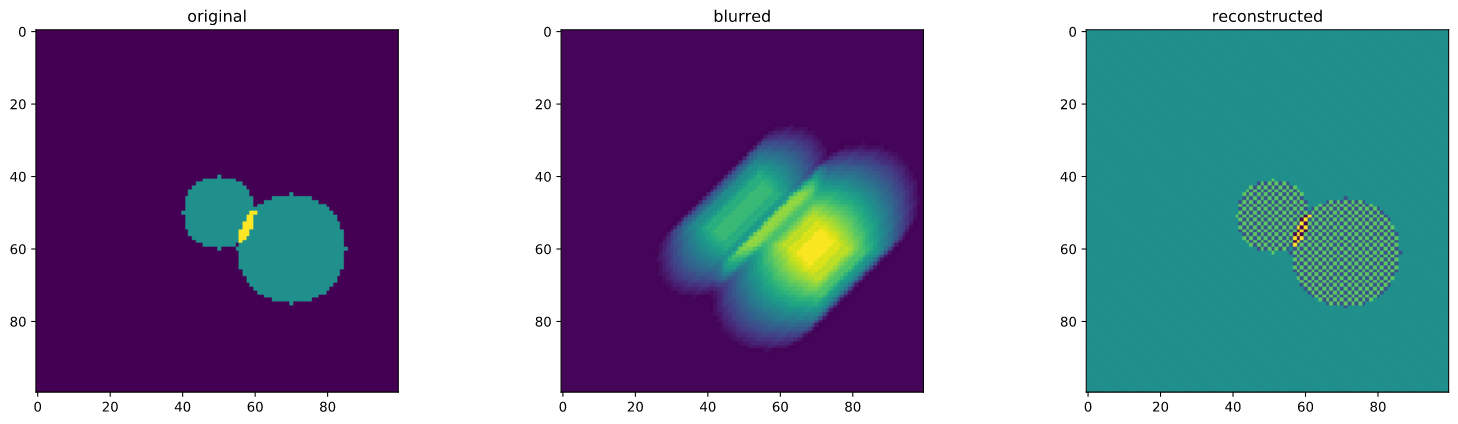
\includegraphics[width=0.75\textwidth]{images/deconvolution.png}
  \end{figure}

\subsubsection{Important transformations}
Both Fourier and Laplace make a few operations much simpler. 
They turn differentiations and exponentials into algebraic terms, and convolutions into products.
As such they are very popular in differential equations,
because you can transform a differential equation to Fourier/Laplace domain, solve for the desired function algebraically
instead of having to solve the actual differential equation, and then transform back.
Laplace is more popular in the differential equation world because it works for non-stable systems, too,
whereas Fourier assumes that the system never explodes at any point.

\begin{figure}[h]
  \caption{Important Fourier transformations}
  \centering
    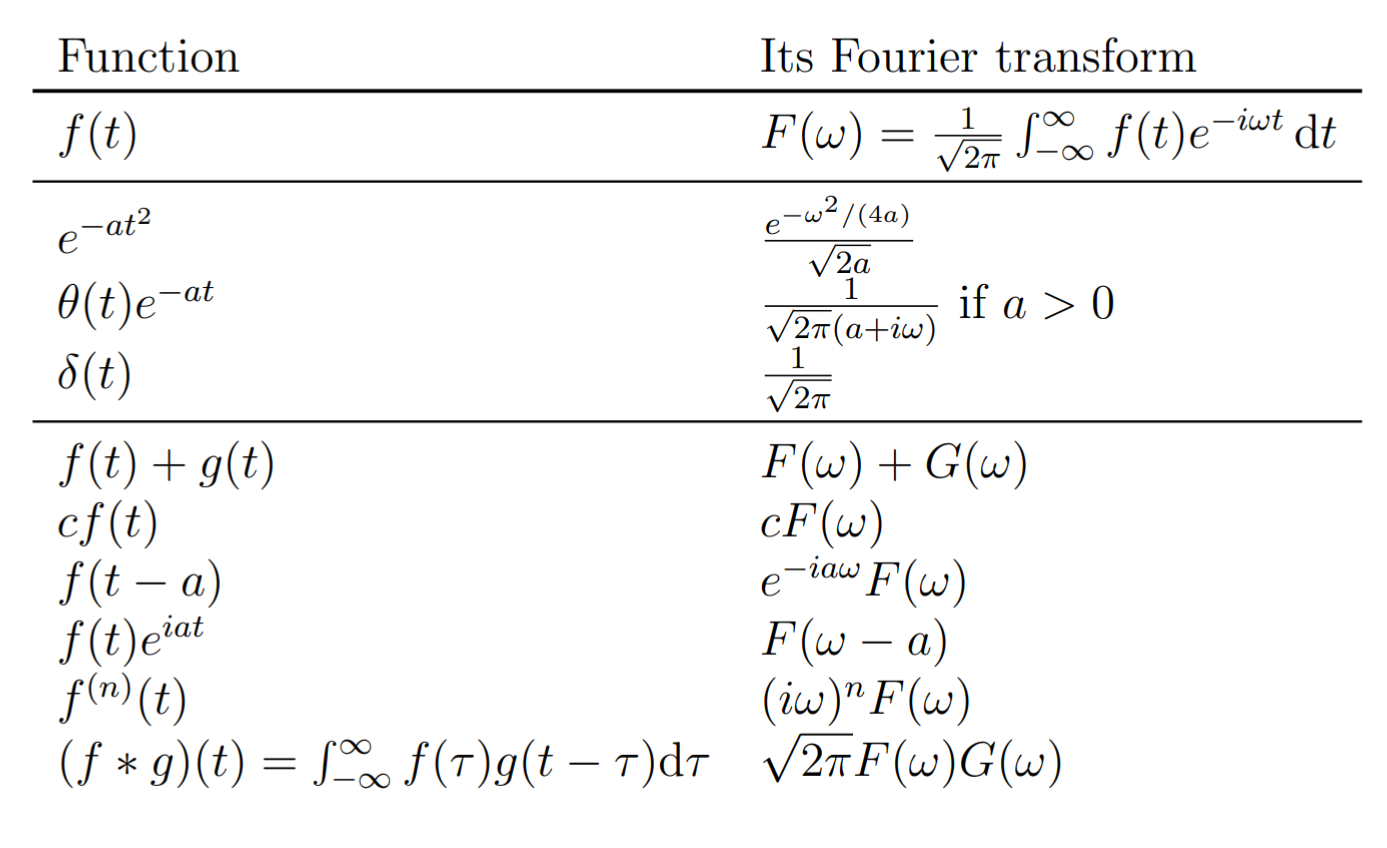
\includegraphics[width=0.75\textwidth]{images/fourier_transforms.png}
\end{figure}

\begin{figure}[h]
    \caption{Important Laplace transformations}
    \centering
      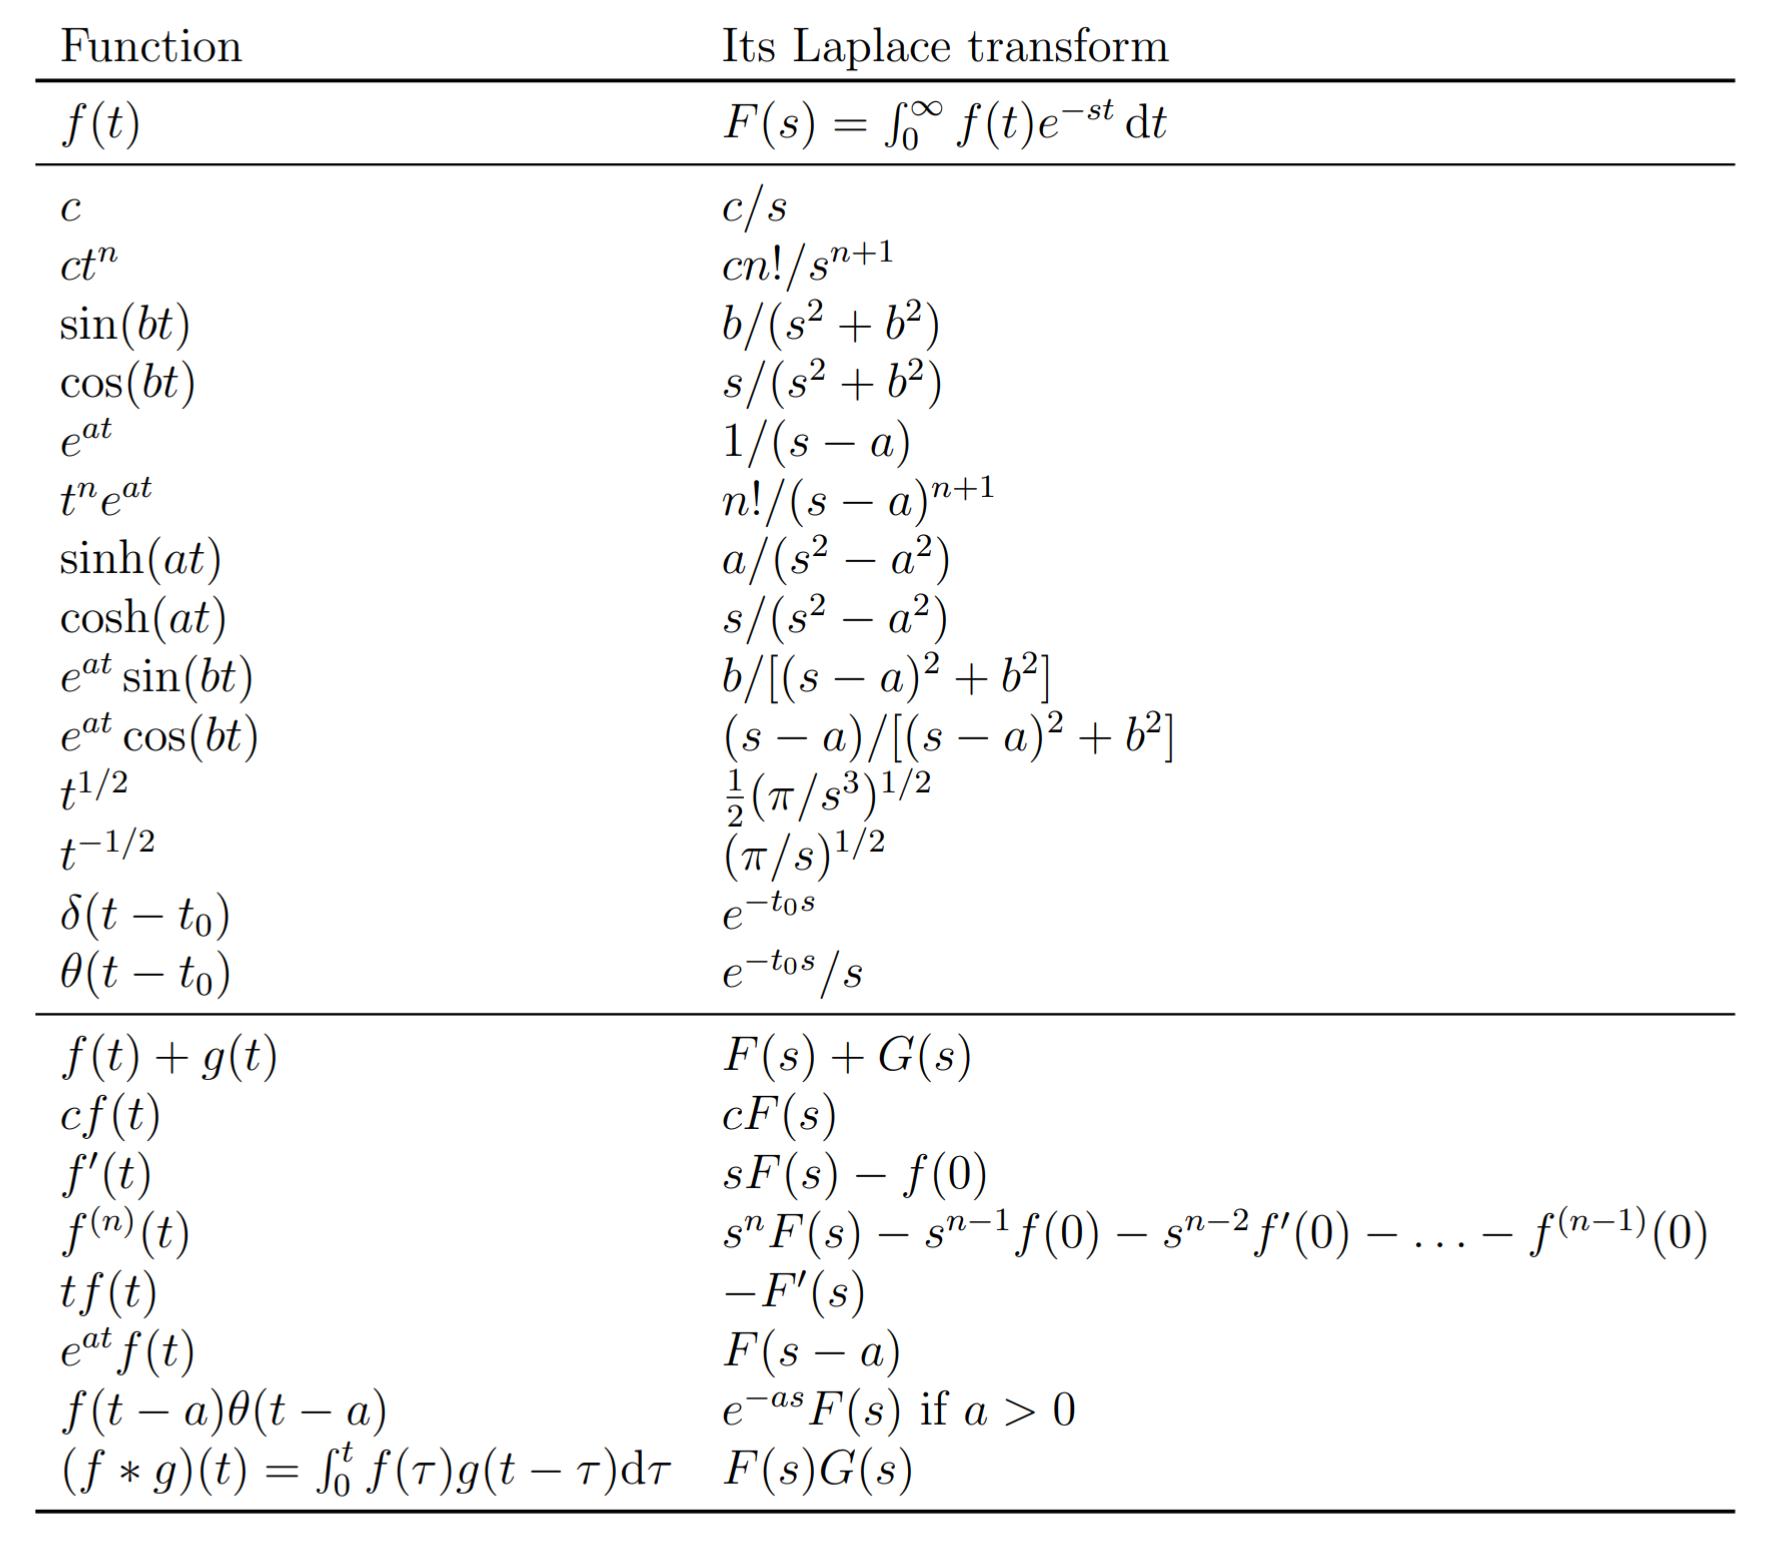
\includegraphics[width=0.7\textwidth]{images/laplace_transforms.png}
\end{figure}

